%!TEX root = report.tex
\subsection{Bus Stop Locations and Routes}
\par The TFL Open Data provides network information on the location of all bus stops in London, and the sequence of bus stops in every bus route.

<<<<<<< Updated upstream
\par This data is in the comma-separated values (CSV) format. We imported the bus sequences into the delay\_bus\_sequences table (Table \ref{table:delay_bus_sequences})

\begin{table}
\centering
\begin{tabular}{@{}llr@{}} \toprule
Column Name & Type & Comments\\ \midrule
id(Primary Key) & int(11)  & Auto Increment\\
route & varchar(64) &  The route name\\
run & int(11) & The route direction\\
sequence & int(11) & The sequence of the bus stop in the route\\
stop\_code\_lbsl & varchar(64) & The internal bus stop identifier\\
bus\_stop\_code & varcher(64) & The public code for the bus stop\\
naptan\_atco & varchar(64) & The national identifier of the bus stop\\
stop\_name & varchar(64) & The name of the bus stop\\ \bottomrule
\end{tabular}
\caption{delay\_bus\_sequences Table Schema}
\label{table:delay_bus_sequences}
\end{table}
 \todo[inline, color=cyan]{Question: Can I skip some columns of the table schema, as those columns have not been used in the project, but just storing as reference for now?}
\par Additionally, we extracted information on all pairs of neighbouring bus stops and the routes that serve between them. We save this information in the delay\_neighbours table (Table \ref{table:delay_neighbours}). See sample data in Table \ref{table:sample_neighbours_view}.

\begin{table}
\centering
\begin{tabular}{@{}llr@{}} \toprule
Column Name & Type & Comments\\ \midrule
id(Primary Key) & int(11)  & Auto Increment\\
route & varchar(64) & The bus route \\
start\_stop & varchar(64) & The stop\_code\_lbsl for the start stop\\
end\_stop & varcher(64) & The stop\_code\_lbsl for the end stop\\ \bottomrule
\end{tabular}
\caption{delay\_neighbours Table Schema}
\label{table:delay_neighbours}
\end{table}

\begin{table}
\centering
\begin{tabular}{@{}llrr@{}} \toprule
id & route & start\_stop & end\_stop \\ \midrule
18433 & 30 & 10002 & 11469 \\
44878 & N19 & 10002 & 11469 \\
47128 & N41 & 10002 & 29772 \\
8653 & 19 & 10002 & 11469 \\ \bottomrule
\end{tabular}
\caption{Sample data in delay\_neighbours Table}
\label{table:sample_neighbours_view}
\end{table}

\subsubsection{Finding the average travel time between neighbouring stops}
\todo[inline] {update this part}
\par To experiment with the queries, we selected one pair of the neighbouring stops (10002, 11469), and listed the time required to travel from stop 10002 to stop 11469 by finding the difference in arrival times for each journey. Sample entries of this list is shown in Figure \ref{fig:journey_time_10002}.

\begin{figure}
\centering
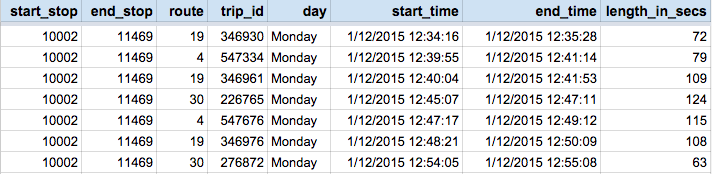
\includegraphics[width=0.7\textwidth]{figures/journey_time_10002.png}
\caption{\label{fig:journey_time_10002} List of journey time from stop 10002 to stop 11469}
\end{figure}


\par We then calculated the average journey time required to travel from 10002 to 11469 for each hour in each week of the day. This information is stored as a timetable, which would be used for further analysis.

Figure\ref{fig:timetable_10002} shows the timetable generated. Each cell indicates the average journey time required to travel from stop 10002 to stop 11469 at a give hour of a give week of day. The \textbf{NULL} values are due to a current databases performance issue. This will be resolved later.

\begin{figure}
\centering
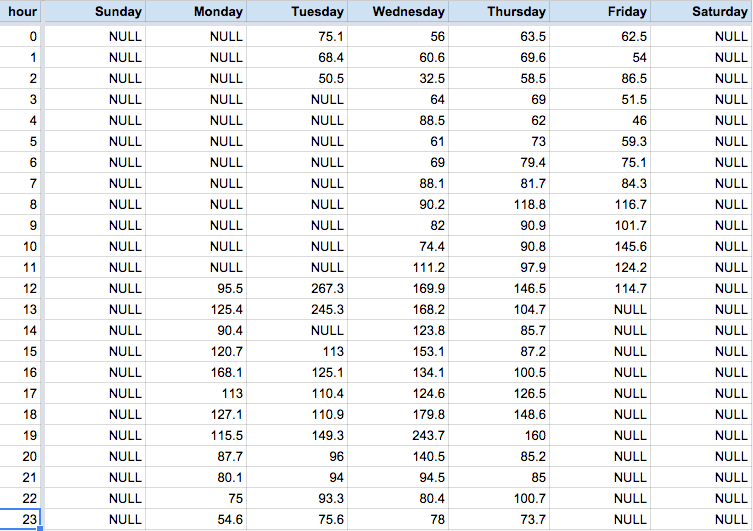
\includegraphics[width=0.9\textwidth]{figures/timetable_10002.png}
\caption{\label{fig:timetable_10002} Average journey time in seconds from stop 10002 to stop 11469 for each hour of each day of week}
\end{figure}

\par We plan to construct a timetable this way for each pair of the neighbouring bus stop.
=======
\par This data is in the comma-separated values (CSV) format.
>>>>>>> Stashed changes
